%!TEX program = xelatex
%!TEX options=--shell-escape

\documentclass[aspectratio=169]{beamer}

\usepackage{pdfpages}

\setbeamerfont{title}{series=\bfseries}
\setbeamerfont{frametitle}{series=\bfseries}

\definecolor{oxford-blue}{HTML}{002147}
\definecolor{oxford-gold}{RGB}{207, 122, 48}

\definecolor{oxford-blue}{RGB}{0,33,71}
\setbeamercolor{title}{fg=oxford-blue}
\setbeamercolor{frametitle}{fg=oxford-blue}
\setbeamercolor{section in toc}{fg=black}
\setbeamercolor{description item}{fg=black}
\setbeamertemplate{description item}{\bfseries\insertdescriptionitem}
\setbeamertemplate{itemize item}{\color{oxford-blue}$\blacktriangleright$}
\setbeamerfont{block title}{series=\bfseries}
\setbeamercolor{block title}{use={frametitle},fg=frametitle.fg,bg=frametitle.bg}

\AtBeginSection[]{
  \begin{frame}
    \vfill\centering\usebeamerfont{title}\insertsectionhead\par\vfill
  \end{frame}
}

\newcommand{\hl}[1]{\textcolor{oxford-blue}{\textbf{#1}}}

\usepackage{fontspec}
\setmonofont[Scale=MatchUppercase]{Fira Mono}
\setsansfont{FoundrySterling}[
  UprightFont=*-Book,
  BoldFont=*-Bold,
  ItalicFont=*-BookItalic
]

\usetheme{default}
\usefonttheme[onlymath]{serif}

\beamertemplatenavigationsymbolsempty

\usepackage{graphicx}
\usepackage{pgffor}
\usepackage{hyperref}
\usepackage{booktabs, colortbl}

\usepackage{tikz}
\usetikzlibrary{positioning, decorations.pathreplacing, fit, calligraphy, arrows.meta, backgrounds, shapes.callouts, shadows.blur, calc}

\usepackage[export]{adjustbox}
\title{
  
\includegraphics[height=18mm]{../../backtracer}\\~\\%
  A NetLogo extension for data provenance
}
\date{\scriptsize\today}
\author{Nicolas Payette}
\institute{%
  
\includegraphics[height=8mm]{geog-brand-pos}%
  
\includegraphics[height=8mm]{ox_brand_cmyk_pos.eps}
}
\titlegraphic{\textcolor{oxford-blue!85}{\url{https://payette.io}}}

\begin{document}

\maketitle

\section{A bit of context}

{
\setbeamercolor{background canvas}{bg=}
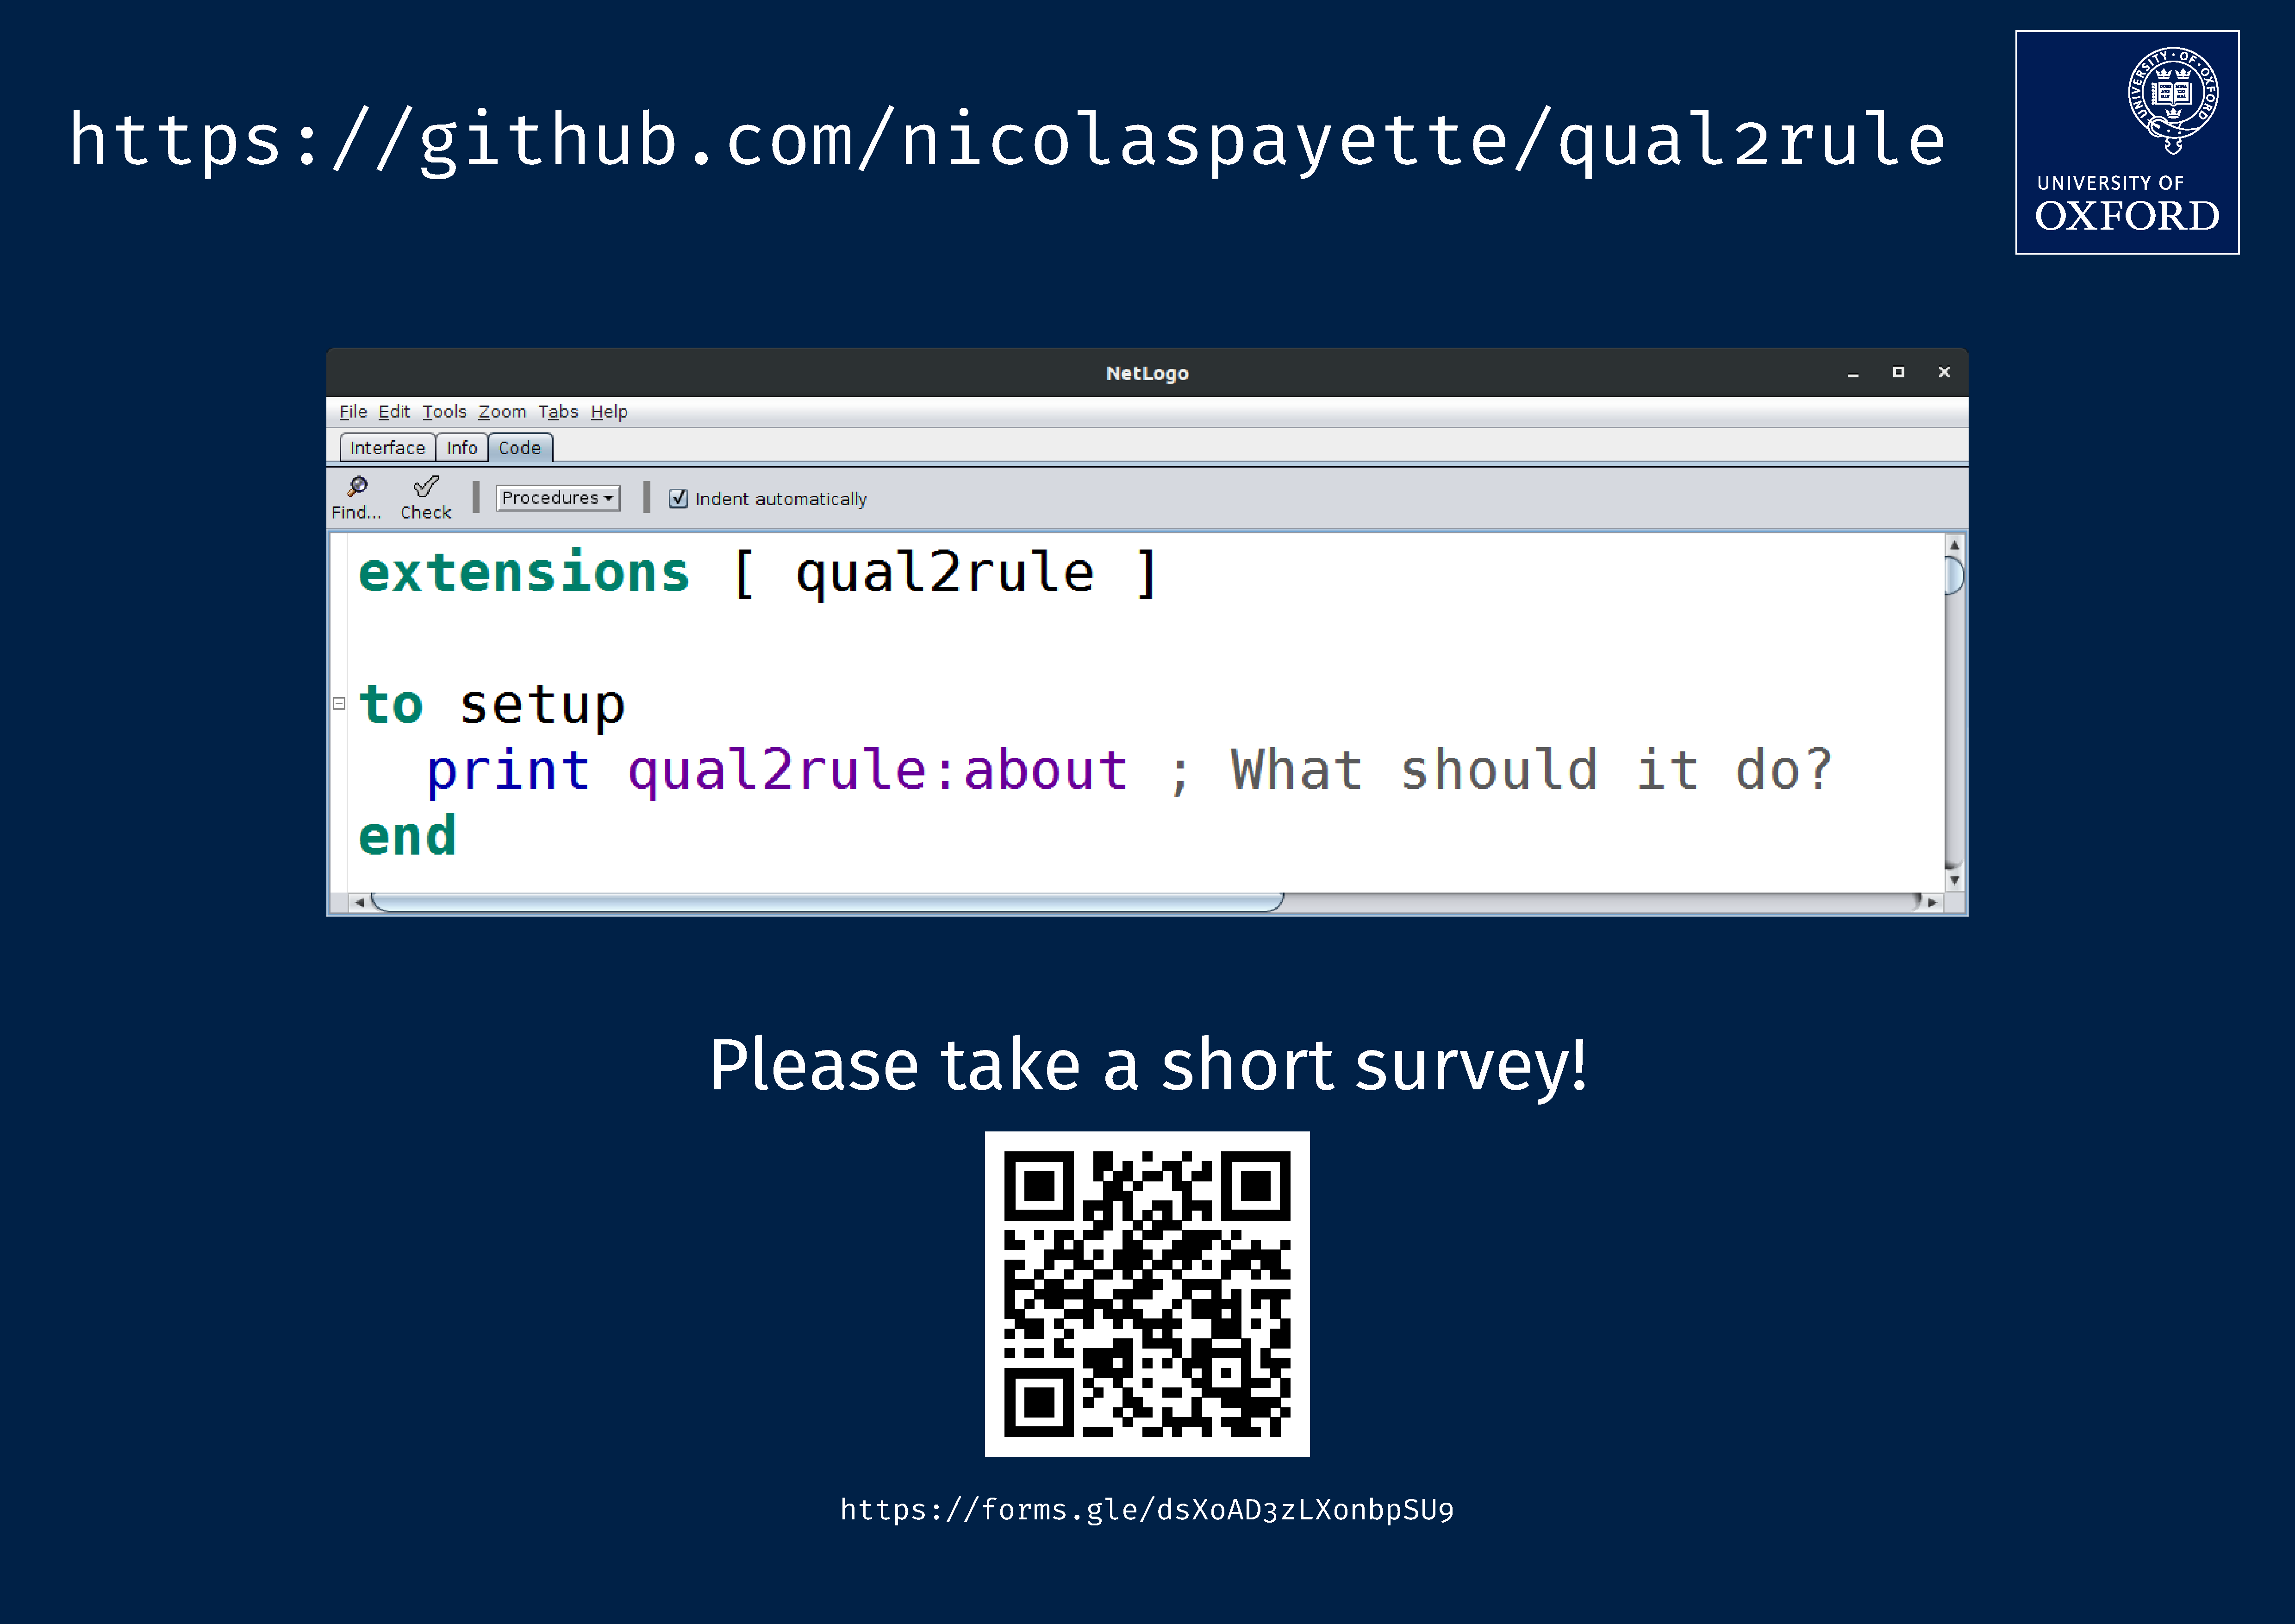
\includepdf[pages=1]{../poster/poster.pdf}
}

\tikzset{
  decoration = {calligraphic brace, amplitude = 10pt},
  backfont/.style = {font=\Large\bf, text=black!50},
  box/.style = {
    semithick, draw, rounded corners = 6pt, align = center
  },
  frontbox/.style = {
    box, fill=oxford-gold!10, draw=oxford-gold, text width = 30mm, minimum height=1.8cm, font=\Large
  },
  backbox/.style = {
    box, fill=oxford-blue!5, draw=oxford-blue!40, inner sep=4mm, backfont
  },
  output/.style = {input},
  arrow/.style = {very thick, -{Stealth[scale=1.25]}, draw=black!60},
  fatarrow/.style = {ultra thick, -{Stealth[scale=1.25]}, draw=oxford-blue},
  hl/.style = {font=\bf, text=oxford-blue},
  bracelabel/.style = {midway, xshift=-7mm, text width=5cm, anchor=center, rotate=90, backfont, align = center}
}

\newcommand{\Brace}[2]{
  \node [fit=#2] (#1-brace) {};
  \draw [decorate, very thick, color=black!70] (#1-brace.south west) -- (#1-brace.north west) node [bracelabel] {#1};
}

\newcommand{\adaptedview}[1]{
  \begin{adjustbox}{max height=.85\textheight}
    \begin{tikzpicture}[
      wideback/.style = {backbox, minimum width = 95mm},
      analbox/.style = {frontbox, fill=black!1, draw=black!50}
    ]
      \node [analbox] (quantianal) {Quantitative\\analysis};
      \node [analbox, right = 2cm of quantianal] (qualianal) {Qualitative\\analysis};
      \begin{scope}[on background layer]
        \node [wideback, fit=(quantianal)(qualianal)] (anal) {};
        \Brace{Analysis}{(anal)}
      \end{scope}
      \node [frontbox, above = 15mm of quantianal] (formalmodels) {Formal\\models};
      \node [frontbox, above = 15mm of qualianal] (semiformalmodels) {Semi-formal\\models};
      \begin{scope}[on background layer]
        \node [wideback, fit=(formalmodels)(semiformalmodels)] (modelbox) {};
        \Brace{Models}{(modelbox)}
      \end{scope}
      \node [frontbox, above = of modelbox] (code) {NetLogo\\code};
      \begin{scope}[on background layer]
        \node [wideback, fit=(code)] (codebox) {};
        \Brace{Simulation}{(codebox)}
      \end{scope}
      \node [frontbox, below = of anal] (raw) {``Raw'' data};
      \begin{scope}[on background layer]
        \node [wideback, fit=(raw)] (data) {};
        \Brace{Data}{(data)}
      \end{scope}
      #1
    \end{tikzpicture}
  \end{adjustbox}
}

\begin{frame}[t]\frametitle{Qualitative survey data}
  \vfill\centering
  \resizebox{.75\textwidth}{!}{$n=7$}
  \vfill
\end{frame}

\newcommand{\whatshoulditdo}[2]{
  \frametitle{\large In your ideal world, what would a \texttt{qual2rule} NetLogo extension do?}
  \begin{columns}[c]
    \begin{column}{0.625\textwidth}
      \LARGE
      #1
      \vfill
    \end{column}
    \begin{column}{0.375\textwidth}
      \adaptedview{#2}
    \end{column}
  \end{columns}
}

\begin{frame}[fragile]{The big picture}
  \begin{center}
    \adaptedview{
      \node [wideback, below = of raw] (phenom) {Phenomena};
      \draw [arrow] (phenom) -- (raw);
      \draw [arrow] (raw) -- (quantianal);
      \draw [arrow] (raw) -- (qualianal);
      \uncover<2>{
        \draw [arrow] (quantianal) -- (formalmodels);
        \draw [arrow] (qualianal) -- (semiformalmodels);
        \draw [arrow] (qualianal) -- (formalmodels);
        \draw [arrow] (semiformalmodels) -- (formalmodels);
        \draw [arrow] (formalmodels) -- (code);
      }
    }
  \end{center}
\end{frame}

\begin{frame}
  \whatshoulditdo{\normalsize
    \begin{itemize}
      \item ``link bits of code to some text (maybe in Infotab) and back again? Or...  faciltates some of the qualitative analytic frameworks to  aid  translation into code''
      \item ``Provide data traceability (e.g. link specific theory, to specific qualitative data, to specific model specification, to specific agent behaviour).''
      \item ``Help with systematic documentation of data use (especially of the qualitative data). Here, maybe something can be done to extend the ODD protocol.''
      \item ``Possibly provide a kind of link to qualitative data analysis software (e.g. Nvivo, Atlas.ti) in a similar way a link to GIS and R is provided.''
    \end{itemize}
  }{
    \draw [fatarrow, {Stealth[scale=1.25]}-{Stealth[scale=1.25]}] (code) -- (formalmodels);
    \draw [fatarrow, {Stealth[scale=1.25]}-{Stealth[scale=1.25]}] (code) -- (semiformalmodels);
    \draw [fatarrow, {Stealth[scale=1.25]}-{Stealth[scale=1.25]}] (code) -- (raw);
    \draw [fatarrow, {Stealth[scale=1.25]}-{Stealth[scale=1.25]}] (formalmodels) -| ([xshift=-25mm]raw);
    \draw [fatarrow, {Stealth[scale=1.25]}-{Stealth[scale=1.25]}] (semiformalmodels) -| ([xshift=25mm]raw);
  }
\end{frame}
